\documentclass{beamer}
%Information to be included in the title page:

\usetheme{Berlin}
\usepackage[slovene]{babel}
\usepackage{ragged2e}
%\usepackage{graphicx}


\title{1. domača naloga}
\subtitle{Napredna računalniška orodja}
\author{Anže Jarc}
\institute{Fakulteta za strojništvo}
\date{2023}
\logo{

\includegraphics[height=1cm]{Slike/logo.png}
}

\begin{document}

\frame{\titlepage}
\begin{frame}
    \frametitle{Kazalo}
    \tableofcontents
\end{frame}

  
\AtBeginSection[]
{
  \begin{frame}
    \frametitle{Kazalo}
    \tableofcontents[currentsection]
  \end{frame}
}

\section{Matlab}

\begin{frame}
\frametitle{Programska in funkcijska datoteka}
\justifying
Cilj naloge je bil izračunati število $\pi$ na podlagi razmerja naključnih točk v krogu in izven njega. Izračune smo opravili v programskem okolju Matlab, kjer smo ukaze shranili v programski in funkcijski datoteki.

V programski datoteki je zapisano zaporedje ukazov, ki se izvršijo ko poženemo program. V programski datoteki ponavadi kličemo funkcije, ki so zapisane v funkcijksi datoteki. Razlika med programskimi in funkcijskimi datotekami je, da so spremenljivke v programski datoteki globalne, v funkcijski pa lokalne.
\end{frame}

\begin{frame}






\frametitle{Anonimna funkcija in vizualizacija}
\begin{columns}
% Column 1
\begin{column}{0.5\textwidth}
\justifying
        Anonimna funkcija sestoji iz samo enega ukaza, a je kljub temu uporabna saj za njeno definicijo ne potrebujemo funkcijske datoteke.
\end{column}
% Column 2    
\begin{column}{0.5\textwidth}
    \begin{figure}
    \centering
        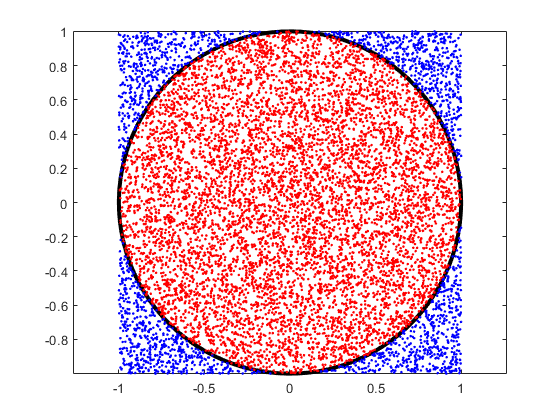
\includegraphics[width=1\textwidth]{Slike/Graf pi.png}
        \caption{10000 naključnih točk.}
    \end{figure}
\end{column}
\end{columns}




\end{frame}

\section{Git}

\begin{frame}
\frametitle{Git hub}
\justifying
Ko je bil program spisan smo na GitHub repozitorij naložili programsko in funkcijsko datoteko. Nato smo kolegu, ki nas je povabil v njegov repozitorij s pull request grafu dodali primeren naslov, legendo in poimenovanje osi. 

Na GitHub smo naložili tudi to predstavitev, potem ko smo jo končali.
\end{frame}


\section{Beamer}

\begin{frame}
\frametitle{Beamer predstavitev}

Predstavitev je morala vsebovati:
\begin{itemize}
    \item Naslovnico, kazalo in logotip fakultete.
\pause
    \item Tekst in vsaj eno sliko s podnapisom.
\pause
    \item Funkcijo \textit{\textbackslash}\textit{pause}
\end{itemize}
\end{frame}



\end{document}